\chapter{Arhitektura i dizajn sustava}
		
		\textbf{\textit{dio 1. revizije}}\\

		\textit{ Potrebno je opisati stil arhitekture te identificirati: podsustave, preslikavanje na radnu platformu, spremišta podataka, mrežne protokole, globalni upravljački tok i sklopovsko-programske zahtjeve. Po točkama razraditi i popratiti odgovarajućim skicama:}
	\begin{itemize}
		\item 	\textit{izbor arhitekture temeljem principa oblikovanja pokazanih na predavanjima (objasniti zašto ste baš odabrali takvu arhitekturu)}
		\item 	\textit{organizaciju sustava s najviše razine apstrakcije (npr. klijent-poslužitelj, baza podataka, datotečni sustav, grafičko sučelje)}
		\item 	\textit{organizaciju aplikacije (npr. slojevi frontend i backend, MVC arhitektura) }		
	\end{itemize}

	
		

		

				
		\section{Baza podataka}
			
			
		Za potrebe našeg sustava koristit ćemo SQL relacijsku bazu podataka. Relacijska baza podataka najviše nam odgovara zbog olakšanog modeliranja događaja i entiteta iz stvarnog svijeta. Osnovna jedinka baze podataka je relacija, to jest tablica koja ima svoj naziv i potreban skup atributa. Zadaća baze podataka je brza i jednostavna pohrana, izmjena i dohvat podataka koje potom treba obraditi. Sve su relacije u bazi svedene na treću normalnu formu kako baza ne bi sadržavala redundantne podatke. Prilikom izrade baze podataka poslužili smo se PostgreSQL-om.
		Baza podataka ove aplikacije sastoji se od sljedećih entiteta:
		\begin{itemize}
			\item 	Profil
			\item 	KorisničkiRačun
			\item 	Uloga
			\item   TipUloge
			\item   Klijent
			\item   Djelatnik
			\item   Bankar
			\item   Administrator
			\item   SlužbenikZaOdobravanjeKredita
			\item   Banka
			\item   Kredit
			\item   Transakcija
			\item   Račun
			\item   VrstaRačuna
			\item   TekućiRačun
			\item   ŠtedniRačun
			\item   ŽiroRačun
			\item   Kartica
			\item   VrstaKartice
			\item   DebitnaKartica
			\item   KreditnaKartica
			\item   Kamata		
		\end{itemize}
		
			\subsection{Opis tablica}
			

				\textbf{Profil} Ovaj entitet sadrži sve važne informacije za pristup web aplikaciji. Sadrži atribute: ime, prezime, OIB, korisničko ime, adresa prebivališta, datum rođenja, e-mail adresa, slika profila i broj tipa uloge. Ovaj entitet u vezi je \textit{Zero-to-Many} s entitetom Korisnički račun preko korisničkog imena.  
				
				\begin{longtabu} to \textwidth {|X[6, l]|X[6, l]|X[20, l]|}
					
					\hline \multicolumn{3}{|c|}{\textbf{Profil }}	 \\[3pt] \hline
					\endfirsthead
					
					\hline \multicolumn{3}{|c|}{\textbf{Profil}}	 \\[3pt] \hline
					\endhead
					
					\hline 
					\endlastfoot
					
					\cellcolor{LightGreen}Ime & VARCHAR	&  	ime korisnika 	\\ \hline
					Prezime	& VARCHAR &  prezime korisnika 	\\ \hline 
					OIB & INT &  OIB korisnika \\ \hline 
					Korisničko ime & VARCHAR	&  	jedinstveni identifikator korisnika	\\ \hline 
					Adresa prebivališta & VARCHAR &   adresa korisnika      \\ \hline
					Datum rođenja & DATE & datum rođenja korisnika \\ \hline
					Email & VARCHAR & e-mail adresa korisnika \\ \hline
					Slika & LONGBLOB & slika korisnika \\ \hline
					Tip uloge & INT & broj tipa uloge \\ \hline
					 
					
					
				\end{longtabu}
			
			\textbf{Korisnički Račun}  Ovaj entitet sadrži sve važne informacije vezane za korisnički račun koji je dodijeljen svakom korisniku koji želi koristiti ovu web aplikaciju. Sadrži atribute: Korisničko ime, lozinku, OIB, ime i prezime korisnika te broj tipa uloge. Ovaj je entitet u vezi \textit{Many-to-Zero} s entitetom Profil preko korisničkog imena i u vezi \textit{One-to-One} s entitetom Uloga preko korisničkog imena.  
			
			\begin{longtabu} to \textwidth {|X[6, l]|X[6, l]|X[20, l]|}
				
				\hline \multicolumn{3}{|c|}{\textbf{Korisnički račun }}	 \\[3pt] \hline
				\endfirsthead
				
				\hline \multicolumn{3}{|c|}{\textbf{Korisnički račun}}	 \\[3pt] \hline
				\endhead
				
				\hline 
				\endlastfoot
				
				\cellcolor{LightGreen}Korisničko ime & VARCHAR	&  jedinstveni identifikator korisnika ( profil.korisničko ime) 	\\ \hline
				Lozinka	& VARCHAR &   hash lozinke	\\ \hline 
				OIB & INT & OIB korisnika (profil.oib)  \\ \hline
				Ime & VARCHAR &  ime korisnika (profil.ime)  \\ \hline 
				Prezime & VARCHAR	& prezime korisnika 		\\ \hline 
				\cellcolor{LightBlue} Tip uloge	& INT &  broj tipa uloge(profil.tip uloge) 	\\ \hline 
				
				
			\end{longtabu}
		
		\textbf{Uloga}  Ovaj entitet sadrži sve važne informacije vezane za ulogu koji je dodijeljen svakom korisniku koji želi koristiti ovu web aplikaciju. Sadrži atribute: Korisničko ime i broj tipa uloge. Ovaj je entitet u vezi \textit{One-to-One} s entitetom Korisnički račun preko korisničkog imena, u vezi \textit{One-to-One} s entitetom Tip Uloge preko broja tipa uloge.  
		
		\begin{longtabu} to \textwidth {|X[6, l]|X[6, l]|X[20, l]|}
			
			\hline \multicolumn{3}{|c|}{\textbf{Uloga}}	 \\[3pt] \hline
			\endfirsthead
			
			\hline \multicolumn{3}{|c|}{\textbf{Uloga}}	 \\[3pt] \hline
			\endhead
			
			\hline 
			\endlastfoot
			
			Korisničko ime & VARCHAR & Korisničko ime korisnika  \\ \hline
			\cellcolor{LightGreen}Tip uloge & INT	&  Broj tipa uloge	\\ \hline
		
			
			 
			
			
		\end{longtabu}
	
		
			
		\textbf{Tip uloge}  Ovaj entitet sadrži informacije vezane za tipove uloge. Sadrži atribute: broj tipa uloge i naziv uloge. Ovaj je entitet u vezi \textit{One-to-One} s entitetom Uloga preko broja tipa uloge.  
		
		\begin{longtabu} to \textwidth {|X[6, l]|X[6, l]|X[20, l]|}
			
			\hline \multicolumn{3}{|c|}{\textbf{Uloga}}	 \\[3pt] \hline
			\endfirsthead
			
			\hline \multicolumn{3}{|c|}{\textbf{Uloga}}	 \\[3pt] \hline
			\endhead
			
			\hline 
			\endlastfoot
			
		    Broj uloge & INT & Broj tipa uloge  \\ \hline
			\cellcolor{LightGreen}Naziv & VARCHAR	& Naziv uloge	\\ \hline
			
			
			
			
			
		\end{longtabu}
	
		\textbf{Klijent} Ovaj entitet sadrži sve važne informacije vezane za klijenta. Sadrži atribute: ime, prezime, OIB, korisničko ime, lozinka, adresa prebivališta, datum rođenja, email, spol i slika. Ovaj entitet je u vezi \textit{One-to-Many} s entitetom Račun preko korisničkog imena, u vezi \textit{One-to-Many} s entitetom Kartica preko korisničkog imena korisnika. 
	
	\begin{longtabu} to \textwidth {|X[6, l]|X[6, l]|X[20, l]|}
		
		\hline \multicolumn{3}{|c|}{\textbf{Klijent}}	 \\[3pt] \hline
		\endfirsthead
		
		\hline \multicolumn{3}{|c|}{\textbf{Klijent}}	 \\[3pt] \hline
		\endhead
		
		\hline 
		\endlastfoot
		
			\cellcolor{LightGreen}Ime & VARCHAR	&  	ime klijenta 	\\ \hline
			Prezime	& VARCHAR &  prezime klijenta 	\\ \hline 
			OIB & INT &  OIB klijenta \\ \hline 
			Korisničko ime & VARCHAR	&  	jedinstveni identifikator korisnika	\\ \hline 
			Lozinka & VARCHAR & hash lozinke \\ \hline
			Adresa prebivališta & VARCHAR &   adresa klijenta      \\ \hline
			Datum rođenja & DATE & datum rođenja klijenta \\ \hline
			Email & VARCHAR & e-mail adresa korisnika \\ \hline
			Spol & VARCHAR(1) & spol klijenta \\ \hline
			Slika & LONGBLOB & slika korisnika \\ \hline
		
		
		
		
	\end{longtabu}

		\textbf{Djelatnik}  Ovaj entitet sadrži sve važne informacije koje su potrebne za djelatnika. Sadrži atribute: ime, prezime, OIB, korisničko ime, lozinku, adresu prebivališta, datum rođenja, e-mail, spol i broj tipa djelatnika te broj poslovnice banke. Ovaj entitet je u vezi \textit{Many-to-One} s entitetom Banka preko broja poslovnice banke u kojoj djelatnik radi. 
		
		\begin{longtabu} to \textwidth {|X[6, l]|X[6, l]|X[20, l]|}
			
			\hline \multicolumn{3}{|c|}{\textbf{Djelatnik}}	 \\[3pt] \hline
			\endfirsthead
			
			\hline \multicolumn{3}{|c|}{\textbf{Djelatnik}}	 \\[3pt] \hline
			\endhead
			
			\hline 
			\endlastfoot
			
			\cellcolor{LightGreen}Ime & VARCHAR	&  	ime djelatnika 	\\ \hline
			Prezime	& VARCHAR &  prezime djelatnika 	\\ \hline 
			OIB & INT &  OIB djelatnika \\ \hline 
			Korisničko ime & VARCHAR	&  	jedinstveni identifikator djelatnika	\\ \hline 
			Lozinka & VARCHAR & hash lozinke \\ \hline
			Adresa prebivališta & VARCHAR &   adresa klijenta      \\ \hline
			Datum rođenja & DATE & datum rođenja klijenta \\ \hline
			Email & VARCHAR & e-mail adresa korisnika \\ \hline
			Spol & VARCHAR(1) & spol klijenta \\ \hline
			Tip djelatnika & INT & Broj tipa uloge \\ \hline
			Broj banke & INT & Broj poslovnice banke\\ \hline
			
		
			
			
			
			
		\end{longtabu}
	
			\textbf{Bankar}    Ovaj entitet sadrži sve važne informacije za bankara. Sadrži sve atribute koje sadrži djelatnik te dodatno: broj tipa uloge i broj transakcije koje je proveo. Ovaj entitet u vezi je \textit{One-to-One} s entitetom djelatnik preko korisničkog imena bankara. Entitet bankar u vezi je i s entitetom Transakcija i Klijent vezom \textit{} preko broja transakcije. Isto tako, bankar je u vezi \textit{Many-to-Many} s entitetom Kredit preko broja kredita. Bankar je u vezi \textit{Many-to-One} s entitetom Administrator preko broja nadređenog bankaru.
			
			\begin{longtabu} to \textwidth {|X[6, l]|X[6, l]|X[20, l]|}
				
				\hline \multicolumn{3}{|c|}{\textbf{Bankar}}	 \\[3pt] \hline
				\endfirsthead
				
				\hline \multicolumn{3}{|c|}{\textbf{Bankar}}	 \\[3pt] \hline
				\endhead
				
				\hline 
				\endlastfoot
			
				Korisničko ime & VARCHAR	&  	jedinstveni identifikator bankara	\\ \hline 
				Broj tipa djelatnika & INT & broj tipa djelatnika \\ \hline
				Broj transakcije & INT & broj transakcije \\ \hline
				Broj kredita & LONG & Broj kredita koji ugovara\\ \hline
				Broj nadređenog & INT & broj tipa djelatnika nadređenog bankaru\\ \hline
				
				
				
				
				
			\end{longtabu}
		
		\textbf{Administrator}    Ovaj entitet sadrži sve važne informacije o administratoru. Administrator je zadužen za dodjeljivanje korisničkih računa i uloga bankara i službenika za odobravanje kredita. Sadrži atribute: korisničko ime, tip djelatnika i broj poslovnice banke. U vezi je \textit{Many-to-One} s entitetom Banka preko broja poslovnice banke u kojoj radi i u vezi \textit{One-to-Many} s entitetima Bankar i Službenik za odobravanje kredita preko broja tipa djelatnika.
		
		\begin{longtabu} to \textwidth {|X[6, l]|X[6, l]|X[20, l]|}
			
			\hline \multicolumn{3}{|c|}{\textbf{Administrator}}	 \\[3pt] \hline
			\endfirsthead
			
			\hline \multicolumn{3}{|c|}{\textbf{Administrator}}	 \\[3pt] \hline
			\endhead
			
			\hline 
			\endlastfoot
			
		 
			Korisničko ime & VARCHAR	&  	jedinstveni identifikator administratora	\\ \hline 
			Tip uloge & INT & broj tipa uloge \\ \hline
			Broj tipa djelatnika & INT & broj tipa djelatnika
			
			
			
			
		\end{longtabu}
	
		
				\textbf{Službenik za odobravanje kredita}   Ovaj entitet sadrži sve važne informacije koje su potrebne za ulogu službenika za odobravanje kredita. Sadrži atribute: korisničko ime, broj tipa uloge, broj poslovnice banke, broj nadređenog i broj kredita koji odobrava ili odbija. U vezi je \textit{Many-to-One} s entitetom Administrator preko broja tipa djelatnika nadređenog službeniku za odobravanje kredita. U vezi je \textit{Many-to-Many} s entitetom kredit preko broja kredita koji odobrava ili odbija. 
		
		\begin{longtabu} to \textwidth {|X[6, l]|X[6, l]|X[20, l]|}
			
			\hline \multicolumn{3}{|c|}{\textbf{Službenik za odobravanje kredita}}	 \\[3pt] \hline
			\endfirsthead
			
			\hline \multicolumn{3}{|c|}{\textbf{Službenik za odobravanje kredita}}	 \\[3pt] \hline
			\endhead
			
			\hline 
			\endlastfoot
			
			Korisničko ime & VARCHAR	&  	jedinstveni identifikator službenika	\\ \hline 
			Tip uloge & INT & broj tipa uloge\\ \hline
			Broj nadređenog & INT & broj tipa djelatnika nadređenog službeniku za odobravanje kredita\\ \hline
			Broj kredita & LONG & broj kredita\\ \hline
			
			
			
			
		\end{longtabu}
	
					\textbf{Banka}   Ovaj entitet sadrži sve važne informacije o poslovnici u kojoj rade djelatnici određene banke. Sadrži atribute: broj banke, naziv banke i adresa banke. U vezi je \textit{One-to-Many} s entitetom Djelatnik preko broja poslovnice banke i u vezi je \textit{Many-to-Many} s entitetom Kredit preko broja kredita koji daje određenom klijentu.  
			
			\begin{longtabu} to \textwidth {|X[6, l]|X[6, l]|X[20, l]|}
				
				\hline \multicolumn{3}{|c|}{\textbf{Banka}}	 \\[3pt] \hline
				\endfirsthead
				
				\hline \multicolumn{3}{|c|}{\textbf{Banka}}	 \\[3pt] \hline
				\endhead
				
				\hline 
				\endlastfoot
				
				Broj poslovnice & INT & broj poslovnice \\ \hline
				Adresa & VARCHAR & adresa banke \\ \hline
				Naziv & VARCHAR & naziv banke \\ \hline
				Broj kredita & LONG & broj kredita\\ \hline
				
				
				
				
			\end{longtabu}
		
			\textbf{Kredit}   Ovaj entitet sadrži sve važne informacije o kreditu koji klijent zatraži. Sadrži atribute: broj kredita, iznos, vrsta kredita, datum ugovaranja i vremenski period otplate kredita.U vezi je \textit{Many-to-One} s entitetom Bankar preko broja kredita i u vezi \textit{Many-to-One} s entitetom Klijent preko broja kredita. Isto tako, entitet Kredit u vezi je \textit{Many-to-One} s entitetom Službenik za odobravanje kredita preko broja kredita.
		
		\begin{longtabu} to \textwidth {|X[6, l]|X[6, l]|X[20, l]|}
			
			\hline \multicolumn{3}{|c|}{\textbf{Kredit}}	 \\[3pt] \hline
			\endfirsthead
			
			\hline \multicolumn{3}{|c|}{\textbf{Kredit}}	 \\[3pt] \hline
			\endhead
			
			\hline 
			\endlastfoot
			
			Broj kredita & LONG & broj kredita \\ \hline
			Iznos & DECIMAL (10, 2) & iznos kredita \\ \hline
			Vrsta & VARCHAR & vrsta kredita \\ \hline
			Datum ugovaranja & DATE & datum ugovaranja kredita \\ \hline
			Vremenski period otplate & INT & duljina otplate kredita \\ \hline
			
			
			
			
		\end{longtabu}
	
		
				\textbf{Transakcija}   Ovaj entitet sadrži sve važne informacije o transakcijama koje klijent želi provesti. Sadrži atribute: broj transakcije, broj računa terećenja, račun odobrenja, datum transakcije, iznos i ukupno stanje. Entitet Transakcija u vezi je \textit{Many-to-One} s entitetom Klijent preko broja transakcije i u vezi \textit{Many-to-One} s entitetom Bankar preko broja transakcije. Isto tako u vezi je \textit{Many-to-One} s entitetom Račun preko broja računa terećenja i broja računa odobrenja.
			
			\begin{longtabu} to \textwidth {|X[6, l]|X[6, l]|X[20, l]|}
				
				\hline \multicolumn{3}{|c|}{\textbf{Transakcija}}	 \\[3pt] \hline
				\endfirsthead
				
				\hline \multicolumn{3}{|c|}{\textbf{Transakcija}}	 \\[3pt] \hline
				\endhead
				
				\hline 
				\endlastfoot
				
				Broj transakcije & INT & broj transakcije \\ \hline
				Račun terećenja & INT & broj računa terećenja \\ \hline
				Račun odobrenja & INT & broj računa odobrenja \\ \hline
				Datum transakcije & DATE & datum transakcije \\ \hline
				Iznos & DECIMAL (10, 2) & iznos uplate \\ \hline
				Ukupno stanje & DECIMAL (10, 2) & ukupno stanje nakon transakcije \\ \hline
				
				
				
				
				
				
			\end{longtabu}
		
			\textbf{Račun}   Ovaj entitet sadrži sve važne informacije o računu koji ima klijent. Sadrži atribute: broj računa, OIB klijenta, datum otvaranja računa, stanje računa i vrsta računa. U vezi je  \textit{Many-to-One} s entitetom Klijent preko OIB-a klijenta. Entitet Račun također je u vezi \textit{Many-to-One} s entitetom Bankar preko korisničkog imena bankara i u vezi je \textit{One-to-Many} s entitetom Kartica preko broja kartice.
		
		\begin{longtabu} to \textwidth {|X[6, l]|X[6, l]|X[20, l]|}
			
			\hline \multicolumn{3}{|c|}{\textbf{Račun}}	 \\[3pt] \hline
			\endfirsthead
			
			\hline \multicolumn{3}{|c|}{\textbf{Račun}}	 \\[3pt] \hline
			\endhead
			
			\hline 
			\endlastfoot
			
			Broj računa & LONG & broj računa \\ \hline
			OIB & INT & OIB klijenta \\ \hline
			Datum otvaranja & DATE & datum otvaranja računa \\ \hline
			Stanje & DECIMAL (10, 2) & trenutno stanje računa \\ \hline
			Korisničko ime bankara & VARCHAR & korisničko ime bankara koji je otvorio račun\\ \hline
			Broj kartice & LONG & broj kartice vezane uz račun\\ \hline
			
			
			
			
			
			
			
		\end{longtabu}
	
				\textbf{Vrsta računa}   Ovaj entitet sadrži sve važne informacije o vrsti računa koje neki klijent posjeduje. Sadrži atribute: broj vrste računa i naziv računa. U vezi je \textit{One-to-Many} s entitetima Tekući račun, Štedni račun i Žiro račun. 
			
			\begin{longtabu} to \textwidth {|X[6, l]|X[6, l]|X[20, l]|}
				
				\hline \multicolumn{3}{|c|}{\textbf{Vrsta računa}}	 \\[3pt] \hline
				\endfirsthead
				
				\hline \multicolumn{3}{|c|}{\textbf{Vrsta računa}}	 \\[3pt] \hline
				\endhead
				
				\hline 
				\endlastfoot
				
				Vrsta računa & INT & Broj vrste računa \\ \hline
				Naziv računa & VARCHAR & Naziv vrste računa \\ \hline
				
				
				
				
				
				
				
			\end{longtabu}
		
		
			\textbf{Tekući račun}   Ovaj entitet sadrži sve važne informacije koje nam trebaju za izgradnju tekućeg računa. Sadrži atribute: broj računa, broj vrste računa i prekoračenje. U vezi je \textit{Many-to-One} s entitetom Račun preko broja računa i u vezi \textit{One-to-One} s entitetom Vrsta računa preko broja vrste računa. 
		
		\begin{longtabu} to \textwidth {|X[6, l]|X[6, l]|X[20, l]|}
			
			\hline \multicolumn{3}{|c|}{\textbf{Tekući račun}}	 \\[3pt] \hline
			\endfirsthead
			
			\hline \multicolumn{3}{|c|}{\textbf{Tekući račun}}	 \\[3pt] \hline
			\endhead
			
			\hline 
			\endlastfoot
			
			Broj računa & LONG & broj tekućeg računa \\ \hline
			Broj vrste računa & INT & broj vrste računa\\ \hline
			Prekoračenje & DECIMAL(10,2) & iznos prekoračenja računa \\ \hline
		
			
			
			
			
			
			
		\end{longtabu}
	
		
			
		\textbf{Štedni račun}   Ovaj entitet sadrži sve važne informacije o štednom računu. Sadrži atribute: broj računa, broj vrste računa. U vezi je \textit{Many-to-One} s entitetom Račun preko broja računa i u vezi \textit{One-to-One} s entitetom Vrsta računa preko broja vrste računa. 
		
		\begin{longtabu} to \textwidth {|X[6, l]|X[6, l]|X[20, l]|}
			
			\hline \multicolumn{3}{|c|}{\textbf{Štedni račun}}	 \\[3pt] \hline
			\endfirsthead
			
			\hline \multicolumn{3}{|c|}{\textbf{Štedni račun}}	 \\[3pt] \hline
			\endhead
			
			\hline 
			\endlastfoot
			
			Broj računa & LONG & broj štednog računa \\ \hline
			Broj vrste računa & INT & broj vrste računa\\ \hline
			Kamatna stopa & DECIMAL(2, 2) & iznos kamatne stope \\ \hline
			Datum zatvaranja & DATE & datum zatvaranja računa \\ \hline
			
			
			
			
			
			
			
			
		\end{longtabu}
	
	\textbf{Žiro račun}    Ovaj entitet sadrži sve važne informacije o žiro računu. Sadrži atribute: broj računa i broj vrste računa. U vezi je \textit{Many-to-One} s entitetom Račun preko broja računa i u vezi \textit{One-to-One} s entitetom Vrsta računa preko broja vrste računa. 
	
	\begin{longtabu} to \textwidth {|X[6, l]|X[6, l]|X[20, l]|}
		
		\hline \multicolumn{3}{|c|}{\textbf{Žiro račun}}	 \\[3pt] \hline
		\endfirsthead
		
		\hline \multicolumn{3}{|c|}{\textbf{Žiro račun}}	 \\[3pt] \hline
		\endhead
		
		\hline 
		\endlastfoot
		
		Broj računa & LONG & broj štednog računa \\ \hline
		Broj vrste računa & INT & broj vrste računa\\ \hline
		
		
		
		
		
		
		
	\end{longtabu}
		
		
			\textbf{Kartica}   Ovaj entitet sadrži sve važne informacije o karticama koje ima klijent. Sadrži atribute: broj kartice, OIB klijenta i broj tipa kartice, stanje i datuma isteka valjanosti kartice. U vezi je \textit{Many-to-One} s entitetom Klijent preko OIB-a klijenta i u vezi \textit{Many-to-One} s entitetom Račun preko broja kartice. U vezi je \textit{One-to-One} s entitetom Vrsta kartice preko broja vrste kartice. 
			
			\begin{longtabu} to \textwidth {|X[6, l]|X[6, l]|X[20, l]|}
				
				\hline \multicolumn{3}{|c|}{\textbf{Kartica}}	 \\[3pt] \hline
				\endfirsthead
				
				\hline \multicolumn{3}{|c|}{\textbf{Kartica}}	 \\[3pt] \hline
				\endhead
				
				\hline 
				\endlastfoot
				
				Broj kartice & LONG & broj kartice\\ \hline
				OIB & INT & OIB klijenta\\ \hline
				Tip kartice & INT & broj tipa kartice\\ \hline
				Stanje & DECIMAL(10,2) & stanje kartice\\ \hline
				Valjanost & DATE & datum isteka valjanosti kartice \\ \hline
	
		

		\end{longtabu}	
	
			\textbf{Vrsta kartice}   Ovaj entitet sadrži sve važne informacije o vrstama kartice koje ima klijent. Sadrži atribute:broj tipa kartice i naziv kartice. U vezi je \textit{One-to-One} s entitetom Kartica preko broja vrste kartice i u vezi \textit{One-to-One} s entitetima Kreditna kartica i Debitna kartica preko broja vrste kartice.
	
			\begin{longtabu} to \textwidth {|X[6, l]|X[6, l]|X[20, l]|}
				
				\hline \multicolumn{3}{|c|}{\textbf{Vrsta kartice}}	 \\[3pt] \hline
				\endfirsthead
				
				\hline \multicolumn{3}{|c|}{\textbf{Vrsta kartice}}	 \\[3pt] \hline
				\endhead
				
				\hline 
				\endlastfoot
		
				Tip kartice & INT & broj tipa kartice\\ \hline
				Naziv kartice & VARCHAR & naziv kartice\\ \hline
		
		
		
		\end{longtabu}
	
				\textbf{Debitna kartica}   Ovaj entitet sadrži sve važne informacije o debitnoj kartici. Sadrži atribute: broj kartice i broj vrste kartice. U vezi je \textit{One-to-One} s entitetom Vrsta kartice preko broja vrste kartice i s entitetom Kartica preko broja kartice.
			
			\begin{longtabu} to \textwidth {|X[6, l]|X[6, l]|X[20, l]|}
				
				\hline \multicolumn{3}{|c|}{\textbf{Debitna kartica}}	 \\[3pt] \hline
				\endfirsthead
				
				\hline \multicolumn{3}{|c|}{\textbf{Debitna kartica}}	 \\[3pt] \hline
				\endhead
				
				\hline 
				\endlastfoot
				
				Broj kartice & LONG & broj kartice\\ \hline
				Broj vrste kartice & INT & broj vrste kartice\\ \hline
				
				
				
				
			\end{longtabu}
	
			\textbf{Kreditna kartica}   Ovaj entitet sadrži sve važne informacije o kreditnoj kartici. Sadrži atribute: broj kartice, broj tipa kartice, trenutno dugovanje, kamatna stopa na iskorišteni limit, odobren limit kartice i iskorišten limit kartice. U vezi je \textit{One-to-One} s entitetom Vrsta kartice preko broja vrste kartice.
			
			\begin{longtabu} to \textwidth {|X[6, l]|X[6, l]|X[20, l]|}
				
				\hline \multicolumn{3}{|c|}{\textbf{Kreditna kartica}}	 \\[3pt] \hline
				\endfirsthead
				
				\hline \multicolumn{3}{|c|}{\textbf{Kreditna kartica}}	 \\[3pt] \hline
				\endhead
				
				\hline 
				\endlastfoot
				
				\cellcolor[LightBlue]{Broj kartice} & LONG & broj kartice\\ \hline
				Broj vrste kartice & INT & broj vrste kartice\\ \hline
				Trenutno dugovanje & DECIMAL(10,2) & trenutno dugovanje\\ \hline
				Kamatna stopa & DECIMAL(2,2) & iznos kamatne stope\\ \hline
				Odobren limit & DECIMAL(10,2) & odobren limit kartice\\ \hline
				Iskorišten limit & DECIMAL(10,2) & iskorišten limit kartice\\ \hline
				
				
				
			\end{longtabu}
		
		
			\textbf{Kamata}   Ovaj entitet sadrži sve važne informacije o kamati kredita. Sadrži atribute: broj kredita, datum uplate, kamatna stopa i mjesečni iznos uplate. U vezi je \textit{One-to-One} s entitetom Kredit preko broja kredita.
		
		\begin{longtabu} to \textwidth {|X[6, l]|X[6, l]|X[20, l]|}
			
			\hline \multicolumn{3}{|c|}{\textbf{Kamata}}	 \\[3pt] \hline
			\endfirsthead
			
			\hline \multicolumn{3}{|c|}{\textbf{Kamata}}	 \\[3pt] \hline
			\endhead
			
			\hline 
			\endlastfoot
			
			Broj kredita & LONG & broj kredita\\ \hline
			Datum uplate & DATE & datum uplate kamate\\ \hline
			Kamatna stopa & DECIMAL(2,2) & Iznos kamatne stope\\ \hline
			Mjesečni iznos & DECIMAL(10,2) & mjesečni iznos uplate\\ \hline
		
			
			
		\end{longtabu}
		
			
			\subsection{Dijagram baze podataka}
				\begin{figure}[H]
					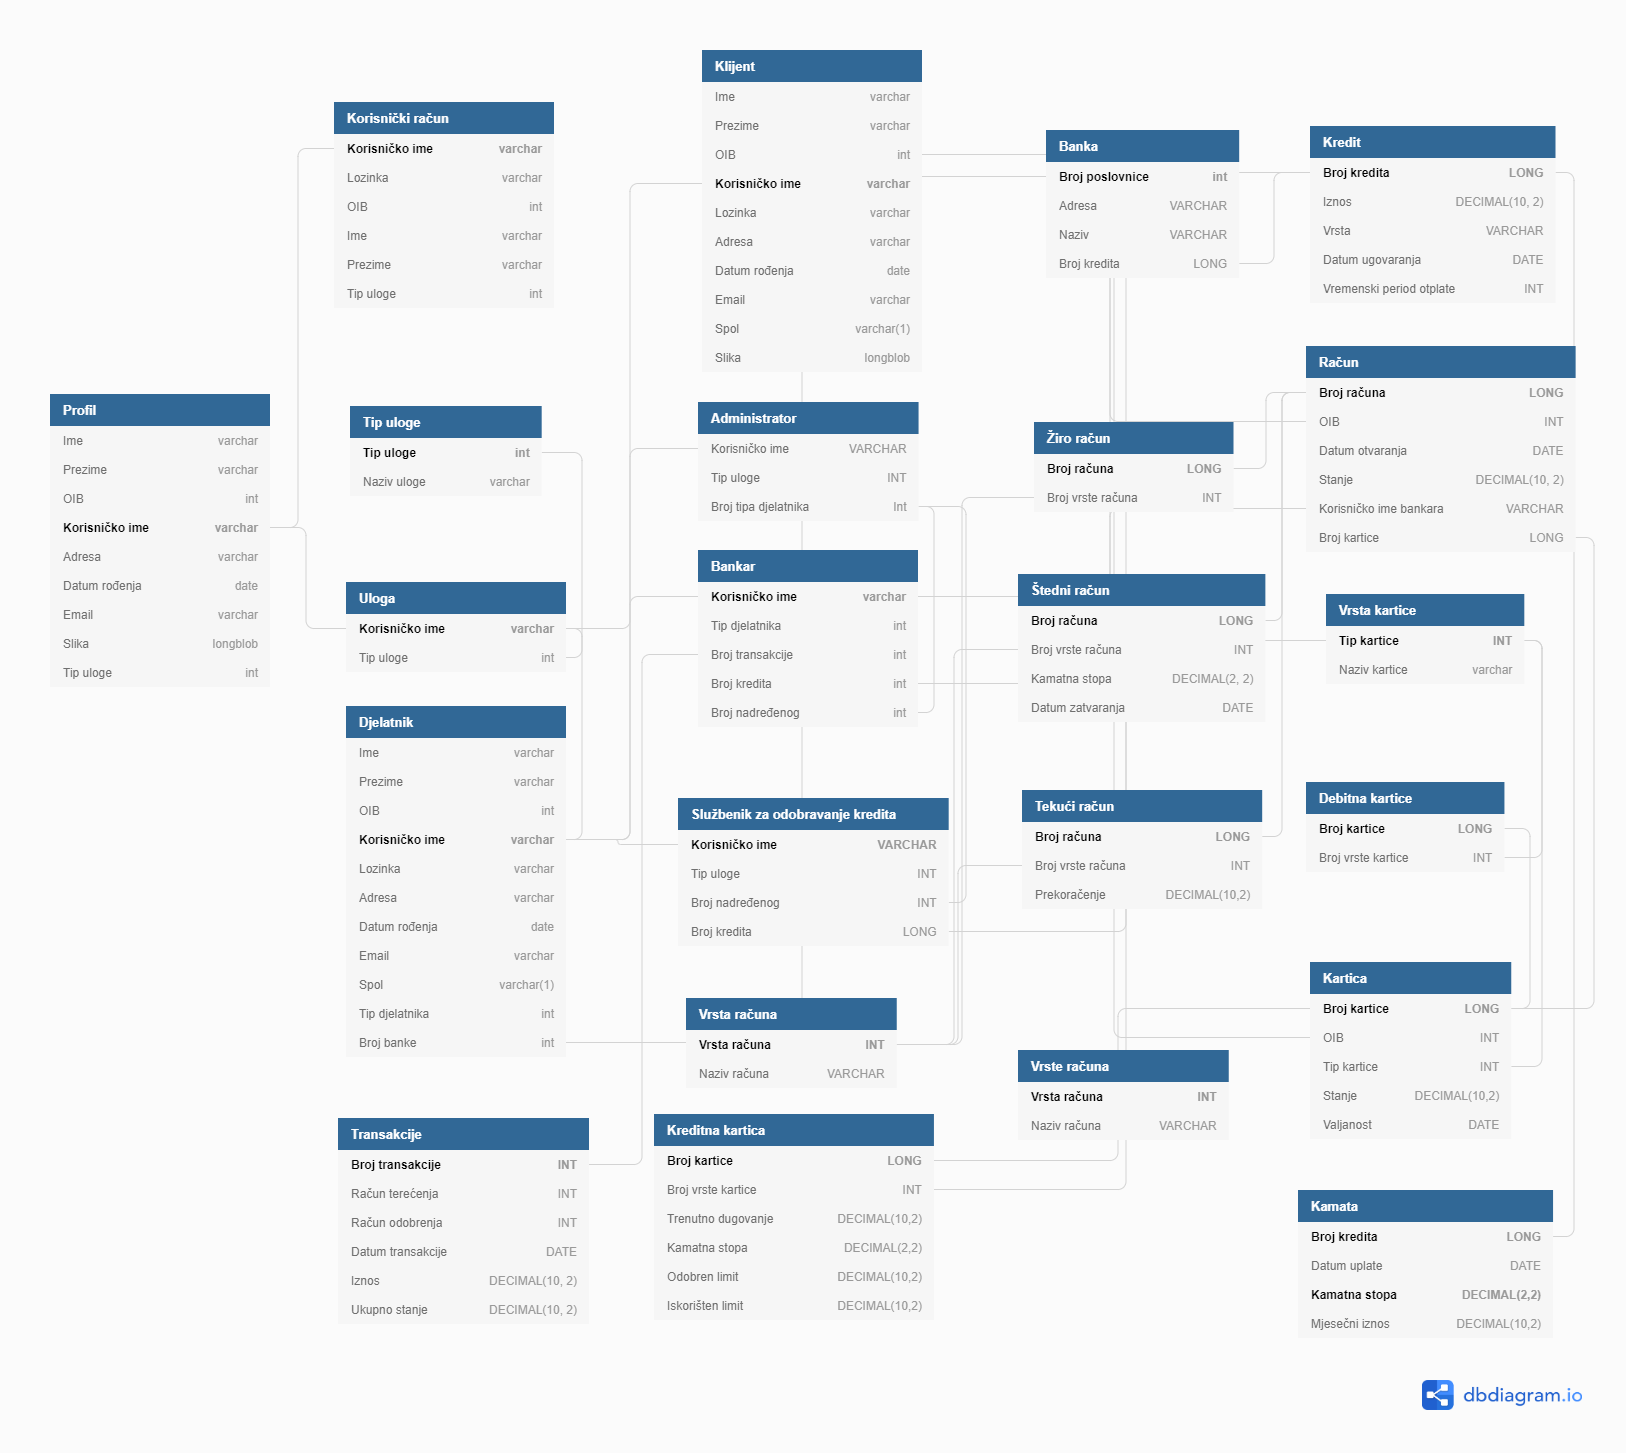
\includegraphics[scale=0.3]{Slike/ER-model.PNG}
					\centering
					\caption{Slika 4.2: E-R dijagram baze podataka}
					\label{fig:dijagram}
				\end{figure}
			\eject
			
			
		\section{Dijagram razreda}
		
			\textit{Potrebno je priložiti dijagram razreda s pripadajućim opisom. Zbog preglednosti je moguće dijagram razlomiti na više njih, ali moraju biti grupirani prema sličnim razinama apstrakcije i srodnim funkcionalnostima.}\\
			
			\textbf{\textit{dio 1. revizije}}\\
			
			\textit{Prilikom prve predaje projekta, potrebno je priložiti potpuno razrađen dijagram razreda vezan uz \textbf{generičku funkcionalnost} sustava. Ostale funkcionalnosti trebaju biti idejno razrađene u dijagramu sa sljedećim komponentama: nazivi razreda, nazivi metoda i vrste pristupa metodama (npr. javni, zaštićeni), nazivi atributa razreda, veze i odnosi između razreda.}\\
			
			\textbf{\textit{dio 2. revizije}}\\			
			
			\textit{Prilikom druge predaje projekta dijagram razreda i opisi moraju odgovarati stvarnom stanju implementacije}
			
			
			
			\eject
		
		\section{Dijagram stanja}
			
			
			\textbf{\textit{dio 2. revizije}}\\
			
			\textit{Potrebno je priložiti dijagram stanja i opisati ga. Dovoljan je jedan dijagram stanja koji prikazuje \textbf{značajan dio funkcionalnosti} sustava. Na primjer, stanja korisničkog sučelja i tijek korištenja neke ključne funkcionalnosti jesu značajan dio sustava, a registracija i prijava nisu. }
			
			
			\eject 
		
		\section{Dijagram aktivnosti}
			
			\textbf{\textit{dio 2. revizije}}\\
			
			 \textit{Potrebno je priložiti dijagram aktivnosti s pripadajućim opisom. Dijagram aktivnosti treba prikazivati značajan dio sustava.}
			
			\eject
		\section{Dijagram komponenti}
		
			\textbf{\textit{dio 2. revizije}}\\
		
			 \textit{Potrebno je priložiti dijagram komponenti s pripadajućim opisom. Dijagram komponenti treba prikazivati strukturu cijele aplikacije.}